\chapter{Les Œuvres Universitaires}

\section{Introduction}
    Notre projet comprend la conception et la réalisation d'une application d'aide à la gestion des ressources de la direction des œuvres universitaires (D.O.U) en général. Celle-ci offre des services de transport, de restauration, de bourse, d'hébergement et d'activités scientifiques, culturelles et sportives. Ces même services lui ont été délégué par l'Office National des œuvres universitaires en fonction de la wilaya où est siégée cette même \acs{D.O.U}.\\
    
    À cet effet, il est nécessaire de présenter ces services en plus des missions la \acs{D.O.U} en tant qu'organisme d'accueil afin de comprendre leurs principales activités.\\

\section{Présentation de la \acs{D.O.U} \cite{dou}}
    Les directions des œuvres Universitaires ont été crée conformément à l'arrêté interministériel du 22 décembre 2004 comportant la fixation de leurs sièges en plus de la liste constituant les résidences universitaires qui leur sont rattachées. Elles sont placées sous la tutelle de l'Office National des œuvres universitaires.\\

    Elles sont chargées de veiller à la gestion des ressources financières et humaines, du bon déroulement et du contrôle des résidences universitaires dont elles sont responsables, de la gestion du transport entre les résidences et les différents établissements de l'enseignement supérieur et de la restauration, de la wilaya dont elles font partie.\\

\section{Missions et activités de la \acs{D.O.U} \cite{onou-arrete}}
    Sa mission est de prendre en charge les différentes activités qui lui sont déléguées par l'Office National des œuvres universitaires qui est lui-même sous la tutelle du ministère de l'enseignement supérieur et de la recherche scientifique.\\
    
    Principalement organiser et gérer les services d'hébergement, de restauration, de bourse, de transport et activités scientifique, culturelles et sportives, de manière à assurer la satisfaction des besoins des étudiants.\\
    
    Plus précisément :
    
    \begin{itemize}\renewcommand{\labelitemi}{$\bullet$}
        \item Veiller à la gestion des moyens matériels et financiers qui lui sont affectés.
        \item Prendre les mesures nécessaires au bon fonctionnement des structures placées sous son autorité.
        \item Veiller à la gestion de son personnel et du personnel des résidences universitaires sous son autorité.
        \item Veiller au bon contrôle rationnelle des moyens mis a la disposition des résidences universitaires sous son autorité.
        \item S'assurer, avec les structures et organismes concernés, du suivi des opérations d'investissement et d'équipement des résidences universitaires sous son autorité.
        \item Soumettre périodiquement des rapports sur le fonctionnement des résidences universitaires sous son autorité.
        \item Participer à la création et au bon suivi de l'application du règlement intérieur des résidences universitaires sous son autorité.
        \item Approuver et suivre le bon déroulement des programmes d'activités scientifiques, culturelles et de loisirs des résidences universitaires sous son autorité.
        \item Passez tout marché et contract en relation avec la restauration et le transport assuré par les résidences universitaires sous son autorité.
        \item Exercer l'autorité hiérarchique sur son personnel.
        \item Nommer les personnels dont le mode de nomination n'est pas prévu.
        \item Ordonner les crédits qui lui sont délégués.
    \end{itemize}

\section{L’organisation de la \acs{D.O.U} \cite{onou-arrete}}
    La direction des œuvres universitaires est composée de 04 départements selon le diagramme suivant :

    \begin{figure}[H]
        \centering
            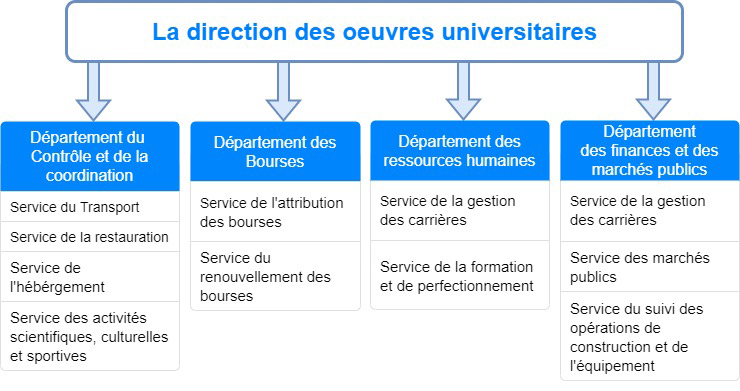
\includegraphics[scale=0.6]{chapitre1/direction-org.jpg}
        \caption{Organigramme de La Direction des Œuvres Universitaires}
    \end{figure}

    Chaque département regroupe plusieurs services qui sont chargé d'assurer différentes fonctions :

    \subsection{Le département du controle et de la coordination}
        \begin{itemize}
            \item Service du transport.
            \item Service de la restauration.
            \item Service de l'hébergement.
            \item Service des activités scientifiques, culturelles et sportives.\\
        \end{itemize}
        
        Il est chargé de :
        \begin{itemize}\renewcommand{\labelitemi}{$\bullet$}
            \item Mettre en œuvre les plans de transport universitaire des résidences universitaires rattachées à la \acs{D.O.U} et superviser le processus jusqu'à son aboutissement.
            \item Superviser, suveiller et orchestrer les actess d'œuvre universitaires assurées par les résidences universitaires associées a la \acs{D.O.U}.
            \item Proposer toute mesure de rationalisation de l'utilisation des moyens humains, matériels et financiers consacrés aux activités des œuvres universitaires.
            \item Examiner les programmes d'activités scientifiques, et sportives et veiller  au suivi de leur application après leur approbation par le directeur de la direction.
        \end{itemize}

    \subsection{Le département des ressources humaines}
        \begin{itemize}
            \item Service de la gestion des carrières.
            \item Service de la formation et de perfectionnement.\\
        \end{itemize}

        Il est chargé de :
        \begin{itemize}\renewcommand{\labelitemi}{$\bullet$}
            \item Gérer la carrière des personnels relevant de ladirectiondes œuvres universitaires.
            \item Assurer la mise en œuvre des plans de formation et du perfectionnement des personnels relevant de la direction des œuvres universitaires.
        \end{itemize}

    \subsection{Le département des bourses}
        \begin{itemize}
            \item Service de l'attribution des bourses.
            \item Service du renouvellement des bourses.\\
        \end{itemize}
        
        Il est chargé de :
        \begin{itemize}\renewcommand{\labelitemi}{$\bullet$}
            \item Assurer le traitement et le suivi des dossiers des étudiants bénéficiaires de bourses.
            \item Assurer le paiement régulier des bourses.
            \item Assurer le traitement et la prise en charge des bourses des étudiants étrangers.
        \end{itemize}

    \subsection{Le département des finances et des marchés publics}
        \begin{itemize}
            \item Service du budget et de la comptabilité.
            \item Service des marchés publics.
            \item Service du suivi des opérations de construction et de l'équipement.\\
        \end{itemize}

        Il est chargé de :
        \begin{itemize}\renewcommand{\labelitemi}{$\bullet$}
            \item Gérer les moyens matériels et financiers mis a la disposition de la direction des œuvres universitaires.
            \item Assurer le service de traitements des personnels de la direction.
            \item Assurer la prise en charge des différents étapes de passation des marchés publics et d'en suivre l'exécution par les résidences universitares.
            \item Assurer en liaison avec les services concernés le suivi des  opérations de construction et d'équipement des résidences universitaires.\\
        \end{itemize}

\section{Les résidences de la direction des œuvres universitaires}
    La \acs{D.O.U} de Tizi Ouzou est composé de résidences:
    \begin{itemize}
        \item Résidence Hasnaoua 1 + 2
        \item Résidence Rehahlia 1 + 2
        \item Résidence Ex Campus Oued Aissi
        \item Résidence Ex Habitat
        \item Résidence Draa Ben Khedda
        \item Résidence Boukhalfa
        \item Résidence Mdouha
        \item Résidence Didouche Mourad
        \item Résidence Tamda 1 + 2 + 3 + 4 + 5 + 7
    \end{itemize}
    Chaque résidence est dotée de plusieurs structures d’accompagnement.\\

\section{Analyse du système}
    Les services de la \acs{D.O.U} effectues plusieurs tâches qui se récapitulent comme suit :

    \subsection*{Hébérgement}
    \begin{itemize}
        \item Effectuer les inscriptions des nouveaux bacheliers reçus. la réinscription des anciens étudiants se fait au niveau de chaque résidence.
        \item Etablissement des listes globales des étudiants et leur répartition par résidence, et par bloc.
        \item Etablissement des statistiques sur l'état d'hébergement des résidences (nombre de places libres, les abandons, ... etc.).
        \item Contrôle des dossiers.
    \end{itemize}

    \subsection*{Transport}
    \begin{itemize}
        \item Assure le transport des étudiants (es) de la Résidence Universitaire vers les campus pédagogiques.
    \end{itemize}

    \subsection*{Réstauration}
    \begin{itemize}
        \item Assurer les repas au étudiants internes et externes.
    \end{itemize}

    \subsection*{Bourse}
    \begin{itemize}
        \item Assurer le traitement et le suivi des dossiers des étudiants bénéficiaires de bourses.
        \item Assurer le renouvellement des bourses.
        \item Assurer le paiement régulier des bourses.
        \item Assurer le traitement et la prise en charge des bourses des étudiants étrangers.
    \end{itemize}

    Parmi les problèmes qui existent après l’analyse de ce système, on peut citer :
    \begin{itemize}
        \item Le transfert de données entre la \acs{D.O.U} et les différentes résidences se fait manuellement.
        \item La répartition des étudiants d’une manière arbitraire, ce qui engendre l’augmentation de l’enveloppe budgétaire alloue au transport. 
        \item La perte de temps.
        \item non disponibilité des informations au bon moment.
        \item La \acs{D.O.U} dispose d'un réseau informatique à haut débit mais très mal exploité. En fait, il n'existe aucune application ou logiciel fonctionnant sous réseau.
        \item L'inconsistance et l'incohérence des informations.\\
    \end{itemize}

\section{Présentation de la solution}
    Afin de remédier aux problèmes cités ci-dessus. Nous avons proposé de concevoir et de réaliser une base de de données répartie en se basant sur la fragmentation horizontale et le développement d'une application de gestion de l'hébergement universitaire permettant de :
    \begin{itemize}
        \item Automatiser les transferts de données.
        \item Affecter les étudiants aux différentes résidences selon le critère de spécialité et nombre de place. 
        \item Assurer un accès facile et rapide aux donnée.
        \item Gagner du temps d'exécution des différents traitements réalisés. Par conséquent, 
        satisfaire les besoins des utilisateurs en matière d'efficacité et de rapidité d'exécution.
        \item Gain financière, en réduisant le nombre de bus de transport universitaire. \\
    \end{itemize}

\section{Conclusion}
    Apres avoir présenté l’organigramme d’accueil et différentes tâches accomplies par le service de l'hébergement nous avons remarqué que ce service souffre de plusieurs problèmes liés particulièrement à une mauvaise gestion de l'hébergement, à savoir principalement, le traitement manuel et la centralisation des données au niveau de la \acs{D.O.U}. Le chapitre suivant sera consacrée à la partie analyse et conception de notre application.\\

\newpage

\leftskip=0cm
\renewcommand{\bibname}{Référence bibliographique et webographique du chapitre 1}
\bibliographystyle{ieeetr}	
\bibliography{chapitre1/chap1}